\documentclass[11pt]{article}
\newcommand{\MODULETAG}{Module 6\,\textbar\,Reporting \& Capstone}
% ===== Toro Resource Estimation Course - shared PDF preamble =====
\usepackage[a4paper,margin=2.4cm,headsep=14pt]{geometry}
\usepackage{amsmath,amssymb}
\usepackage{lmodern}
\usepackage[T1]{fontenc}
\usepackage[utf8]{inputenc}
\usepackage{microtype}
\usepackage{graphicx}
\usepackage{booktabs}
\usepackage{array}
\usepackage{enumitem}
\usepackage{xcolor}
\usepackage{titlesec}
\usepackage{fancyhdr}
\usepackage[most]{tcolorbox}
\usepackage{listings}
\usepackage{caption}
\usepackage[hidelinks]{hyperref}

% ---- palette ----
\definecolor{navy}{HTML}{1F2A44}
\definecolor{navy2}{HTML}{2B3A5C}
\definecolor{bronze}{HTML}{C8702D}
\definecolor{bronzed}{HTML}{A85A1F}
\definecolor{teal}{HTML}{2A7D8C}
\definecolor{tealw}{HTML}{ECF4F5}
\definecolor{ink}{HTML}{26303F}
\definecolor{paper2}{HTML}{F3EDE1}
\definecolor{line}{HTML}{D8D4CB}
\definecolor{codebg}{HTML}{1C2433}
\definecolor{good}{HTML}{3F7D5A}
\definecolor{warn}{HTML}{B4451F}

\color{ink}
\setlength{\parindent}{0pt}
\setlength{\parskip}{6pt}
\linespread{1.06}

% ---- section styling ----
\titleformat{\section}{\Large\bfseries\color{navy}}{\thesection}{0.6em}{}
\titleformat{\subsection}{\large\bfseries\color{navy2}}{\thesubsection}{0.6em}{}
\titleformat{\subsubsection}{\normalsize\bfseries\color{bronzed}}{}{0em}{}
\titlespacing{\section}{0pt}{16pt}{6pt}
\titlespacing{\subsection}{0pt}{12pt}{4pt}

% ---- header / footer ----
\pagestyle{fancy}
\fancyhf{}
\renewcommand{\headrulewidth}{0.4pt}
\renewcommand{\footrulewidth}{0pt}
\fancyhead[L]{\footnotesize\color{navy2}\MODULETAG}
\fancyhead[R]{\footnotesize\color{navy2}Toro Tin Project\,\textbar\,ANRML26-137}
\fancyfoot[C]{\footnotesize\color{navy2}\thepage}

% ---- callout boxes ----
\newtcolorbox{keybox}[1][Key concept]{breakable,enhanced,
  colback=paper2,colframe=bronze,boxrule=0pt,leftrule=4pt,
  arc=2pt,left=10pt,right=10pt,top=8pt,bottom=8pt,
  fonttitle=\bfseries\sffamily\small\color{bronzed},title={#1}}
\newtcolorbox{torobox}[1][Toro application]{breakable,enhanced,
  colback=navy!6,colframe=navy,boxrule=0pt,leftrule=4pt,
  arc=2pt,left=10pt,right=10pt,top=8pt,bottom=8pt,
  fonttitle=\bfseries\sffamily\small\color{navy},title={#1}}
\newtcolorbox{pitbox}[1][Common pitfall]{breakable,enhanced,
  colback=warn!7,colframe=warn,boxrule=0pt,leftrule=4pt,
  arc=2pt,left=10pt,right=10pt,top=8pt,bottom=8pt,
  fonttitle=\bfseries\sffamily\small\color{warn},title={#1}}
\newtcolorbox{notebox}[1][Note]{breakable,enhanced,
  colback=tealw,colframe=teal,boxrule=0pt,leftrule=4pt,
  arc=2pt,left=10pt,right=10pt,top=8pt,bottom=8pt,
  fonttitle=\bfseries\sffamily\small\color{teal},title={#1}}
\newtcolorbox{defbox}[1][Definition]{breakable,enhanced,
  colback=good!7,colframe=good,boxrule=0pt,leftrule=4pt,
  arc=2pt,left=10pt,right=10pt,top=8pt,bottom=8pt,
  fonttitle=\bfseries\sffamily\small\color{good},title={#1}}
\newtcolorbox{objbox}{enhanced,colback=navy,colframe=navy,
  arc=3pt,left=12pt,right=12pt,top=10pt,bottom=10pt,
  coltext=white}

% ---- python code ----
\lstdefinestyle{py}{language=Python,
  basicstyle=\footnotesize\ttfamily\color{white},
  keywordstyle=\color{bronze},commentstyle=\color{line},
  stringstyle=\color{teal!60!white},backgroundcolor=\color{codebg},
  numberstyle=\tiny\color{line},showstringspaces=false,
  breaklines=true,frame=single,framerule=0pt,
  rulecolor=\color{codebg},xleftmargin=8pt,xrightmargin=4pt,
  aboveskip=10pt,belowskip=6pt,framexleftmargin=8pt,
  framexrightmargin=8pt,framextopmargin=6pt,framexbottommargin=6pt}
\lstset{style=py}

% ---- equation box ----
\newtcolorbox{eqbox}{enhanced,colback=white,colframe=line,
  boxrule=0.6pt,arc=2pt,left=8pt,right=8pt,top=4pt,bottom=4pt,
  before skip=10pt,after skip=10pt}

% ---- captions ----
\captionsetup{font={small,it},labelfont={bf,color=navy},labelsep=endash}

% ---- module title macro ----
\newcommand{\moduletitle}[3]{%
  {\sffamily\bfseries\footnotesize\color{bronze}\MakeUppercase{#1}\par}
  \vspace{2pt}
  {\sffamily\bfseries\LARGE\color{navy}#2\par}
  \vspace{3pt}
  {\small\itshape\color{navy2}#3\par}
  \vspace{4pt}{\color{line}\hrule height 1.5pt}\vspace{12pt}}

\begin{document}

\moduletitle{Module 6 of 6}{Block Models, Cut-off Grade and the Resource
Statement}{A kriged grid is not yet a resource --- this module makes it
one, then assesses Toro}

This final module turns estimates into tonnes, applies the economics
that decide what is ore, attaches a classification, and assembles the
formal Resource statement. It closes with a capstone: the honest Toro
resource picture set against the Achmmach and Alphamin Bisie benchmarks.

\begin{objbox}
{\sffamily\bfseries\color{bronze}LEARNING OBJECTIVES}
\begin{itemize}[leftmargin=14pt,itemsep=2pt]
\item Construct a block model and convert estimated grade and volume
into tonnes of ore and metal.
\item Apply the volume-variance relationship.
\item Derive a breakeven cut-off grade and read a grade-tonnage curve.
\item Assign Resource classification to a block model.
\item Assemble a code-compliant Resource statement.
\item Complete the alluvial g/m$^3$ estimate and benchmark Toro.
\end{itemize}
\end{objbox}

\section{The block model}

A \textbf{block model} is the digital orebody: the deposit volume
divided into a regular 3D array of rectangular blocks, each carrying
estimated attributes (grade of every element, density, classification,
rock type, and kriging variance). Block size is a compromise: no smaller
than the data can resolve (typically one quarter to one half of the
drill spacing) and related to the \textbf{selective mining unit} ---
the smallest volume the method can extract as ore or waste separately.
\textbf{Sub-blocking} splits edge blocks where a geological boundary
cuts through them.

\begin{keybox}[Estimate into blocks, never the reverse]
The workflow is strict and one-directional: define domains (Module 3),
model the variogram of each (Module 4), then block-krige each domain into
its blocks (Module 5). Each block's grade is estimated only from samples
in its own domain.
\end{keybox}

\section{From blocks to tonnes}

\begin{eqbox}
\[ T_{\text{block}}=V_{\text{block}}\times\rho,
   \qquad
   M_{\text{block}}=T_{\text{block}}\times\frac{g}{100} \tag{6.1}\]
\end{eqbox}

\subsection*{The volume-variance relationship}

The dispersion variance $D^2(v\,|\,D)$ of grades of volumes $v$ within
deposit $D$ shrinks as $v$ grows. \textbf{Krige's relationship}:

\begin{eqbox}
\[ D^{2}(v\,|\,D) = D^{2}(v\,|\,G) + D^{2}(G\,|\,D) \tag{6.2}\]
\end{eqbox}

The variance of small blocks within a deposit equals their variance
within a panel $G$ plus the variance of panels within the deposit.
Variance partitions cleanly across scales. Selective mining units have a
wider grade distribution than large panels; a model built on the wrong
support will mis-state how much ore sits above cut-off. It is the formal
reason kriging smooths --- a kriged block model cannot reproduce the full
block-scale variance, which is what conditional simulation was created
to fill.

\section{Cut-off grade}

The \textbf{cut-off grade} divides material worth processing from
material that is not. It is fundamentally an economic quantity. The
breakeven (marginal) cut-off is where revenue from treating a tonne as
ore equals processing cost. A tonne at grade $g\%$ contains $g/100$
tonnes of metal:

\begin{eqbox}
\[ \frac{g_c}{100}\times P\times R = C
   \qquad\Longrightarrow\qquad
   g_c = \frac{100\,C}{P\times R} \tag{6.3}\]
\end{eqbox}

A Resource is always reported \textbf{at a stated cut-off}, resting on
realistic, disclosed assumptions for price $P$, recovery $R$ and cost
$C$.

\subsection*{The grade-tonnage curve}

Sweep the cut-off and plot the surviving tonnage and the mean grade of
that tonnage --- the most informative graphic a resource geologist
produces.

\begin{figure}[h]\centering
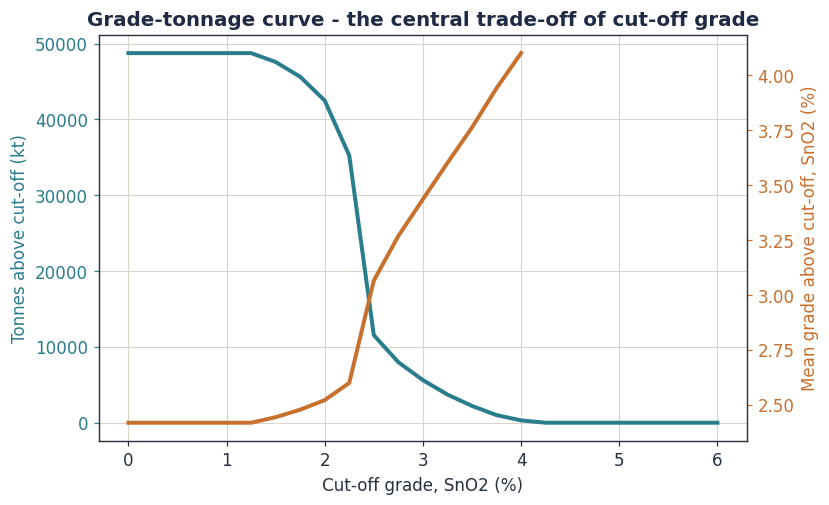
\includegraphics[width=0.78\textwidth]{../assets/figures/fig_gradetonnage.png}
\caption{Toro grade-tonnage relationship. As cut-off rises, tonnage
falls and mean grade rises. Contained metal --- the product --- usually
peaks at a low cut-off and then falls. The ``right'' cut-off maximises
project value, not grade.}
\end{figure}

\section{Classification in practice}

Module 1 defined the categories; here we assign them to blocks.
Evidence: \textbf{drill / pit spacing} (the primary driver),
\textbf{kriging variance} (a direct block-by-block confidence map), the
\textbf{number and configuration of informing samples},
\textbf{conditional simulation} (used to test whether grade in a
production-sized volume is known to a specified tolerance), and
\textbf{geological continuity plus QAQC}.

\begin{pitbox}[The spotted-dog problem]
Classifying purely on a raw kriging-variance threshold scatters isolated
Measured blocks through an Indicated background --- unmineable. The CP
defines confidence as broad, coherent regions, commonly via drill-spacing
criteria validated by conditional simulation, not block by isolated
block.
\end{pitbox}

\section{The Mineral Resource statement}

\begin{center}\small
\begin{tabular}{@{}p{3.4cm}p{3.2cm}p{3.2cm}p{4cm}@{}}
\toprule
\textbf{Classification} & \textbf{Tonnes} & \textbf{Grade} &
\textbf{Contained metal}\\
\midrule
Measured & by domain & \% Sn / g/m$^3$ & tonnes Sn\\
Indicated & by domain & \ldots & \ldots\\
\textbf{Measured + Indicated} & \textbf{subtotal} & \ldots & \ldots\\
Inferred & reported separately & \ldots & \ldots\\
\bottomrule
\end{tabular}
\end{center}

Measured and Indicated are subtotalled because only they can feed a
Reserve; Inferred is always kept separate. The table never travels
alone: it must carry the effective date, cut-off grade and price /
recovery / cost assumptions, the RPEEE basis, and the named CP sign-off.

\begin{keybox}[Rounding is a disclosure]
An Inferred Resource quoted as ``5,234,718 t at 1.07\% Sn'' is
dishonest --- the false precision contradicts the category. ``5.2 Mt at
1.1\% Sn'' tells the truth.
\end{keybox}

\section{Conditional simulation, briefly}

Kriging gives the single best estimate and, by smoothing, deliberately
understates true block-grade variability. \textbf{Conditional simulation}
generates many alternative block models --- \emph{realisations} ---
each of which honours the data and reproduces the real histogram and
variogram. The spread across realisations \emph{is} the uncertainty.

\begin{notebox}[Estimation versus simulation]
Use \textbf{kriging} for the best single estimate --- the resource block
model itself. Use \textbf{conditional simulation} for uncertainty: risk
analysis, classification criteria, grade-control decisions, recoverable
resources. Complementary, not competing.
\end{notebox}

\section{Reconciliation and the path to a Reserve}

Reconciliation compares the resource model, the grade-control model and
what the processing plant actually received --- usually expressed as
mine-call factors. Persistent divergence almost always traces to a
sampling, density, domaining or top-cut problem. Beyond the Resource lies
the Reserve: Measured and Indicated blocks pass into Scoping,
Pre-Feasibility and Feasibility studies that apply the modifying factors
(mining method, dilution, recovery, costs, permits, markets). That is
the journey Achmmach completed to publish 7.0 Mt at 0.82\% Sn Proven and
Probable Reserve.

\section{Completing the alluvial estimate}

The block-model machinery above was demonstrated on the kriged
concentrate grade. A defensible \emph{alluvial} resource is a
volume-grade quantity in g/m$^3$, with the XRF assay supplying only one
factor in equation (2.4):

\begin{eqbox}
\[ g_{\,\mathrm{Sn}}\;\Big[\tfrac{\text{g}}{\text{m}^3}\Big]
   = \frac{M_{\text{HMC}}}{M_{\text{bulk}}} \times a_{\text{Sn}}
   \times \rho_{\text{gravel}} \times 10^{6} \tag{6.4}\]
\end{eqbox}

Applied to the Toro field recoveries (200 kg bulk samples), with mean
concentrate Sn grade $\approx 1.8\%$ and assumed gravel density
1.9 t/m$^3$:

\begin{center}\small
\begin{tabular}{@{}lrr@{}}
\toprule
\textbf{Bulk sample} & \textbf{HMC yield} & \textbf{In-situ Sn (g/m$^3$)}\\
\midrule
Mining Pit (pt 2)     & 1.00\% & 339\\
River Bishwai (pt 13) & 1.00\% & 339\\
Kadade (pt 11)        & 0.50\% & 169\\
Kadade (pt 16)        & 0.50\% & 169\\
GN-005                & 0.18\% &  59\\
\bottomrule
\end{tabular}
\end{center}

Mean $\approx 215$ g/m$^3$ Sn, range 59--339 g/m$^3$ --- an order-of-
magnitude span from just five samples.

\begin{pitbox}[Why the alluvial number is fragile]
Equation (6.4) is a \emph{product}, so the relative errors of its factors
add. A 20\% error in yield, 15\% in concentrate grade and 10\% in density
compound to roughly 27\% in g/m$^3$. The 215 g/m$^3$ mean rests on five
bulk samples, an \emph{assumed} density that has never been measured at
Toro, and a yield read from field washing that had no QAQC. The pitting
programme must deliver, for every pit, a weighed bulk sample of measured
volume, a measured in-situ density, and a logged wash-layer thickness.
Without those, the alluvial estimate cannot rise above an Exploration
Target.
\end{pitbox}

\section{Capstone: the Toro resource picture}

\begin{torobox}[Toro, assessed against this course]
\textbf{Status.} Two distinct Exploration Targets --- an alluvial placer
across Bishiwai, Yadabongo and Kadade, and a primary greisen-pegmatite
target on the LV 029 cupola. Neither is a Mineral Resource, and the
reasons are now precise.

\textbf{Why not yet a Resource.} The grade data resolve to 26 pit
locations (Module 2). The variogram has a relative nugget of 0.55
(Module 4). Cross-validation returns correlation 0.24: unbiased but
imprecise (Module 5). The alluvial g/m$^3$ figure rests on five bulk
samples and an unmeasured density (Module 6).

\textbf{What the data do support.} A real, encouraging signal: structured
grade continuity of roughly 1 km, concentrate grades averaging 2.3\%
SnO$_2$, a reconstructed alluvial grade near 215 g/m$^3$ Sn, and a
coherent higher-grade core through Bishiwai-Yadabongo. Enough to justify
the next tranche of capital --- which is what an Exploration Target is
for.
\end{torobox}

\subsection*{The path from Exploration Target to Mineral Resource}

\begin{center}\small
\begin{tabular}{@{}p{6.4cm}lp{6cm}@{}}
\toprule
\textbf{Action} & \textbf{Modules} & \textbf{What it changes}\\
\midrule
Drill the 13 priority collars; systematic infill pitting & 2, 5 &
Raises density so continuity can be assumed, not implied\\
Designed QAQC stream from the first sample & 2 & Lowers the nugget;
makes the database certifiable\\
Measure in-situ bulk density by domain & 2, 6 & Removes the largest
assumption in tonnage and the g/m$^3$ chain\\
Record wash-layer thickness on every pit & 3, 6 & Enables correct
length-weighted compositing\\
Re-fit variograms per domain; block-krige; classify with QKNA and
simulation & 4--6 & Converts the Exploration Target into a classified
Resource\\
CP sign-off and a code-compliant report & 1, 6 & Makes the Resource
public and bankable\\
\bottomrule
\end{tabular}
\end{center}

\section{The workflow as one chain}

\begin{keybox}[The resource estimation workflow]
\textbf{1.~Foundations} --- know what you are producing, under which
code, and who is accountable. \textbf{2.~Sampling and data} --- collect
representative samples, control the error, certify the database.
\textbf{3.~EDA and statistics} --- understand the distribution and
define the stationary domains. \textbf{4.~Variography} --- measure and
model the spatial continuity of grade. \textbf{5.~Estimation} --- krige
the best linear unbiased estimate, and obtain its quantified uncertainty.
\textbf{6.~Reporting} --- turn estimates into classified tonnes and metal,
honestly. Each module is necessary; none is sufficient alone.
\end{keybox}

Hold on to the deeper lesson, the one the Toro data taught more
forcefully than any clean textbook dataset could. Resource estimation is
not the manufacture of a single confident number. It is the disciplined,
quantified, defensible \emph{statement of what is known and how well it
is known} --- including, when the data demand it, the honest verdict
that the answer is ``not yet, and here is precisely why.'' A geologist
who can deliver that verdict with the rigour of this course, and chart
the path beyond it, is doing resource estimation at the highest level.

\vspace{4pt}{\color{line}\hrule}\vspace{4pt}
{\small\itshape Module 6 closes the Toro Resource Estimation \&
Geostatistics course.}

\end{document}
